% !TEX program = lualatex
% \documentclass[12pt]{ltjsarticle} % 日本語をそのまま扱えるクラス
\documentclass[12pt, leqno]{ltjsarticle}
% \usepackage[margin=28mm]{geometry}
\usepackage{amsmath,amssymb,mathtools}
\usepackage{amsthm}
\usepackage{tikz}
\usetikzlibrary{arrows.meta,positioning,calc}
\usepackage[
  top=15mm,     % 上余白
  bottom=15mm,  % 下余白
  left=10mm,    % 左余白
  right=10mm,    % 右余白
  % landscape,
  margin=10mm
]{geometry}

% ---- 記号・マクロ ----
\newcommand{\xto}{\mathrel{\xrightarrow{}}}
\newcommand{\into}{\hookrightarrow}
\newcommand{\epi}{\twoheadrightarrow}
\newcommand{\pto}{\rightrightarrows}
\newcommand{\cls}[1]{\bigl(#1\bigr)}
\newcommand{\redjoin}{\wedge}
\newcommand{\shrink}{\phi}
\newcommand{\Ex}{E}        % suspension functor E
\newcommand{\Ox}{\Omega}   % loop functor Omega
\newcommand{\id}{\mathrm{id}}
% --- Toda bracket helpers ---
\newcommand{\toda}[1]{\{\,#1\,\}}              % {a,b,c}
\newcommand{\todai}[2][]{\{\,#2\,\}_{#1}}      % {a,b,c}_i   (#1 は添字, 空なら無し) 
\newcommand{\todas}[1]{\langle\,#1\,\rangle}
\newcommand{\gen}[1]{\{\,#1\,\}}       % ⟨generator⟩ 表記を { } で統一
\newcommand{\Ker}{\operatorname{Ker}}
\newcommand{\im}{\operatorname{Im}}
\newcommand{\hs}[2]{\bigl[#1,#2\bigr]}   % 一般のホモトピー集合
\newcommand{\pis}[2]{\pi_{#1}(#2)}       % 左が球面のときのホモトピー群
\newcommand{\pit}[2]{\pi_{#1}^{#2}}
\newcommand{\ext}[1]{\overline{#1}}     % extension
\newcommand{\coext}[1]{\widetilde{#1}}  % coextension
\newcommand{\z}{\mathbb{Z}}
\newcommand{\sq}[1]{Sq^{#1}}
\newcommand{\map}{\operatorname{Map}}

% ---- theorem-like environments ----
\numberwithin{equation}{section}
\theoremstyle{plain}
\newtheorem{theorem}{Theorem}[section]
\newtheorem{lemma}[theorem]{Lemma}
\newtheorem{proposition}[theorem]{Proposition}
\newtheorem{corollary}[theorem]{Corollary}
\theoremstyle{definition}
\newtheorem{definition}[theorem]{Definition}
\newtheorem{example}[]{Example}
\newtheorem{notation}[theorem]{Notation}
\newtheorem{assumption}[theorem]{Assumption}
\theoremstyle{remark}
\newtheorem{remark}[theorem]{Remark}

% \title{PART 1}
% \author{}
% \date{}

\begin{document}
% \maketitle
\begin{center}
  PART 1.
\end{center}

\setcounter{section}{1}

\section*{CHAPTER I\\ General Compositions and Secondary Compositions}

% この章では, 位相空間 $X$ に対して基点 $x_0\in X$ を固定し, 必要に応じて $(X,x_0)$ と書く. 
$n$ 次元単位立方体を
\(
I^n=\{(t_1,\ldots,t_n)\mid 0\le t_i\le 1\}
\)
とし, \\
$(n+1)$ 次元ユークリッド空間内の単位 $n$–球面を, 次で表す.
\[
S^n=\{(t_1,\ldots,t_{n+1})\mid t_1^2+\cdots+t_{n+1}^2=1\}.
\]

% \subsection*{単位立方体から球面への標準写像}
連続写像
\begin{equation}
\psi_n:I^n\longrightarrow S^n
\end{equation}
% \tag{1.1}
を次のように定める. \\
$I^n$ の中心 $c_0=(\tfrac12,\ldots,\tfrac12)$ を,
$S^n$ 上の点 $e_0^*=(-1,0,\ldots,0)$ に, \\
また, 境界 $\partial I^n$ の各点を, 
$e_0=(1,0,\ldots,0)$ に写す.\\
\(x=(t_1,\cdots,t_n)\in\partial I^{n}\)
に対して, 線分
\(\overrightarrow{c_{0}x}\)
を, 大半円
\(\stackrel{\curvearrowright}{e_{0}^{*}e_{0}}\)
に等速で写し,\\
\(e_{0}^{*}\)
での接ベクトルは,
\((0,t_{1},\cdots,t_{n})\)
に平行になるものとする.
\(\psi_n\) は, 以下のような性質を持つ.
\begin{equation}
  \psi_n(\partial I^n) = e_0,\quad
  \psi_n \text{ は, } I^n - \partial I^n \text{ を }
  S^n - e_0 \text{ の上に同相に写す.}
\end{equation}
\[
\psi_n(t) = (\cos 2\pi t,\ \sin 2\pi t).
\]
\(i:S^{n}\hookrightarrow S^{n+1}\)
を,
\(i(s_{0},\cdots,s_{n}) := (s_{0},\cdots,s_{n},0)\)
で定義するとき,
\[
\psi_{n+1}(t_{1},\cdots,t_{n},\frac{1}{2})=
i(\psi_{n}(t_{1},\cdots,t_{n})).
\]
\(\psi_{n}(t_{1},\cdots,t_{n})=(s_{0},\cdots,s_{n})\)
と置く.\\
\(t_{i}\geq\frac{1}{2}\ (t_{i}\leq\frac{1}{2})\)
のとき,
\(s_{i}\geq0\ (s_{i}\leq0)\),\\
\(t_{i}\)
を
\(1-t_{i}\)
に置き換えたとき,
\(s_{i}\)
は
\(-s_{i}\)
に置き換わる.\\
\(t_{i}\)
を
\(t_{j}\)
に置き換えたとき,
\(s_{i}\)
と
\(s_{j}\)
が置き換わる.

以後, 本書では各位相空間 $X$ に対し, 
基点 $x_0\in X$ を固定しておき, 球面の場合は $e_0\in S^n$ を基点にとる. \\
全ての写像と homotopy は基点を保つものとする.\\
i.e.
写像 \(f:X\to Y\),
 homotopy  \(H:X\times I\to Y\)
は, 条件 
\(f(x_0) = y_0\), 
\(H(x_0, t) = y_0,\ (t\in I)\)
を満たす.\\
写像 $f:(X,x_0)\to (Y,y_0)$ の (基点付き) ホモトピー類の集合を,
\[
[X,Y]=\{\, [f]\ \mid\ f:(X,x_0)\to (Y,y_0)\,\}
\]
で表す. 特に, $X=S^n$ のとき,
$[X,Y]$ は通常の $n$ 次ホモトピー群 $\pi_n(Y)$ と一致する. 

% \subsection*{合成 (composition) }
$\alpha\in[X,Y]$, $\beta\in[Y,Z]$ に対して,
それぞれの代表写像を $f:X\to Y$, $g:Y\to Z$ とするとき, \\
合成
\(g\circ f\) は \([X,Z]\) の元を表し,
\(f, g\) の選び方によらない.\\
\(g\circ f\) の類を
\(\beta\circ \alpha \in [X,Z]\)
と書き, \(\alpha\) と \(\beta\) の合成 (composition) という.\\
式 \(\beta\circ \alpha = f^*(\beta) = g_*(\alpha)\)
は, 次の写像を定義する.
\[
f^*:[Y,Z]\to[X,Z],\quad g_*:[X,Y]\to[X,Z].
\]
\[
f^*(\beta)=[g\circ f],\qquad g_*(\alpha)=[g\circ f]
\]
明らかに, 合成は結合的である. 
\[
(\gamma\circ \beta)\circ\alpha=\gamma\circ(\beta\circ\alpha).
\]
\[
(f_2\circ f_1)^*=f_1^*\circ f_2^*,\quad 
(g_2\circ g_1)_*=g_{2*}\circ g_{1*}.
\]

% \subsection*{Reduced join とその基本性質}
二つの基点付き空間 $(A,a_0)$ と $(B,b_0)$ の \emph{reduced join} を, 
$A\ \wedge\ B$ と書き, 積 $A\times B$ の部分集合
\[
A\vee B=\bigl(A\times\{b_0\}\bigr)\cup\bigl(\{a_0\}\times B\bigr)
\]
を, 一点につぶす (shrinking) ことにより得られる空間とする. 
縮約写像 (shrinking map) を,
\[
\shrink_{A,B}:A\times B\longrightarrow
A\times B/A\vee B = A\ \wedge\ B
\]
で表す. 3つの空間 $A,B,C$ に対して, 次の自然な同相がある.
\[
(A\ \wedge\ B)\ \wedge\ C\ \cong\ A\ \wedge\ (B\ \wedge\ C),
\]
\[
\phi_{A\wedge B, C}(\phi_{A,B}(a,b),c)\longleftrightarrow
\phi_{A,B\wedge C}(a, \phi_{B,C}(b,c)).
\]
これにより, $A\ \wedge\ B\ \wedge\ C$ と略記する. 

二つの球面 $S^m$ と $S^n$ の reduced join は,
$S^m\wedge S^n\cong S^{m+n}$ と同一視する.
この同一視を与える写像を
\begin{equation}
\shrink_{m,n}:S^m\times S^n\longrightarrow S^{m+n}
% Toda 原本の (1.3): 縮約写像を表示する番号付き式
\end{equation}
と書く. $(x,y)\in I^m\times I^n=I^{m+n}$ に対して,
\[
\shrink_{m,n}\bigl(\psi_m(x),\,\psi_n(y)\bigr)=\psi_{m+n}(x,y)
\]
で定める.
写像
\[
f:A\to A',\quad g:B\to B'
\]
に対し, reduced join
\[
f\ \wedge \ g:\ A\ \wedge\ B\ \longrightarrow\ A'\ \wedge\ B'
\]
を, 次により自然に定める.
\[
(f\wedge g)\circ \phi_{A,B} = \phi_{A',B'}\circ (f\times g).
\]
次が成り立つ：
\begin{equation}
% \tag{1.4}
\raisetag{3ex}
\begin{aligned}[t]
\text{0).}\ & f\simeq f',\ g\simeq g' \ \Rightarrow\ 
f\ \wedge\ g\simeq f'\ \wedge\ g': A\wedge B\to A'\wedge B',
\qquad\qquad\qquad\qquad\qquad\qquad\\
\text{i).}\ & (f\wedge g)\wedge h = f\wedge (g\wedge h),\\
\text{ii).}\ & (f_2\circ f_1)\ \wedge\ (g_2\circ g_1)\ 
= \ (f_2\ \wedge\ g_2)\circ(f_1\ \wedge\ g_1).
\end{aligned}
\end{equation}

\(f,\ g\) 
を, それぞれ,
\(\alpha\in[A,A'],\ \beta\in[B,B']\)
を表す写像とするとき,\\
(1.4) 0) により,
\(f\wedge g\) 
が表わす類は, 
\(f,g\) の選び方によらない.\\
これを,
\(\alpha\wedge \beta\in[A\wedge B, A'\wedge B']\)
と書き, \(\alpha\) と \(\beta\) の
reduced join と呼ぶ.
(1.4) から, 次が成り立つ.
\begin{equation}
% (1.5)
\raisetag{3ex}
\begin{aligned}[t]
  \text{i).}\ & (\alpha\wedge\beta)\wedge\gamma 
  = \alpha\wedge(\beta\wedge\gamma).\\
  \text{ii).}\ & (\alpha'\circ\alpha)\wedge(\beta'\circ\beta)
  = (\alpha'\wedge\beta')\circ(\alpha\wedge\beta).
  \qquad\qquad\qquad\qquad\qquad\qquad\qquad\qquad\qquad\qquad
\end{aligned}
\end{equation}

% \subsection*{Suspension}
空間 $X$ と $S^n$ の reduced join を,
\[
\Ex^n X\ :=\ X\ \wedge\ S^n
\]
と書き, $X$ の $n$-重 suspension と呼ぶ. 
特に, $n=1$ のときは, 単に $\Ex X=X\ \wedge\ S^1$ と書く. \\
同一視 \(X\wedge S^{m+n} = X\wedge S^m\wedge S^n\)
により, 
\(E^n(E^m X) = E^{m+n} X\) を得る.

写像 $f:X\to Y$ に対し, その $n$–重 suspension
\[
\Ex^n f:\ \Ex^n X\longrightarrow \Ex^n Y,\quad
(Ef = E^1 f)
\]
を, $f\ \wedge\ \id_{S^n}$ により定める. これにより,
\(
\Ex^n(\Ex^m f)=\Ex^{m+n}f
\)
が成り立つ. 
(1.4), (1.5) から次が成り立つ. 
\begin{equation}
% (1.6)
\raisetag{3ex}
\begin{aligned}[t]
  \text{0).}\ 
  & f\simeq g:X\to Y \text{ は, }
  E^n f\simeq E^n g \text{ を導く.}\\
  & [f]\mapsto [E^n f] \text{ は, } 
  E^n : [X,Y] \to [E^n X, E^n Y] \text{ を定める.}\\
  \text{i).}\ 
  & E^n(E^m\alpha) = E^{n+m}\alpha,
  \text{ for } \alpha\in [X,Y].\\
  \text{ii).}\
  & E^n(g\circ f) = E^n g\circ E^n f,\quad
  E^n(\beta\circ\alpha) = E^n\beta\circ E^n\alpha.  
  \qquad\qquad\qquad\qquad\qquad\qquad\qquad
\end{aligned}  
\end{equation}

また, \(X\) の suspension \(EX\) は, 
次の写像によっても定義される.
\[
d_X:X\times I \to EX,\qquad
d_X = \phi_{X,S^1}\circ (1_X\times \psi_1).
\]
ここで, \(1_X\) は \(X\) の恒等写像である.\\
\(d_X\) は, \(X\times \partial{I} \cup x_0 \times I\)
を, \(EX\) の基点へつぶす写像であり, 
これは \(d_X\) を特徴づける.\\
写像 $f:(X,x_0)\to(Y,y_0)$ に対し, 
その suspension $\Ex f:\Ex X\to \Ex Y$ はまた,
次によっても定められる.
\[
\Ex f(d_X(x, t)) = 
d_Y(f(x), t),\quad x\in X,\quad t \in I.
\]

ホモトピー集合 \([EX, Y]\) を考える.\\
写像 $f,g:(\Ex X,x_0)\to(Y,y_0)$ に対し, 
\(f+g,\ -f: (EX,x_0)\to (Y,y_0)\) を, 次で定義する.
\[
(f+g)(d_X(x,t)) :=
\begin{cases}
f(d_X(x,2t)), & 0\le t\le \tfrac12,\\[2mm]
g(d_X(x,2t-1)), & \tfrac12\le t\le 1,
\end{cases}
\]
\[
(-f)(d_X(x, t)) := 
f(d_X(x, 1-t)).
\]
これらの演算 \(+, -\) は, 
 homotopy と compatible であり,
よって, \([EX, Y]\) 上の演算を誘導する.\\
写像 \((X,x_0)\to(Y,y_0)\) の空間 \(Y_0^X\)
の基本群と同様,
この演算により, $[\Ex X,Y]$ は群になる.\\
実際, 
\(X\) が locally compact のとき,
これらは自然に同型となる.
\[
[\Ex X,Y]\cong \pi_1\bigl(Y^X_{0}\bigr).
\]
次の事は容易に得られる.
写像 $f:Y\to Z$ と $g:W\to X$ に対して, 次は準同型である.
\begin{equation}
\label{eq:toda-1-7}
f_*:[EX,Y]\longrightarrow[EX,Z],\qquad
(Eg)^*:[EX,Y]\longrightarrow[EW,Y].
\end{equation}
すなわち,
\[
[f]\circ(\alpha + \alpha') = [f]\circ\alpha + [f]\circ\alpha',
\]
\[
(\alpha + \alpha')\circ E[g] = \alpha\circ E[g] + \alpha'\circ E[g].
\]
特に, $n\ge 2$ のとき,
\([\Ex^n X,Y]\) はアーベル群である.

% \subsection*{球面の場合の $d_n$}
$X=S^n$ のとき, 先の $d_X$ を $d_n$ と書き, 
次で定められる.
\begin{equation}
% (1.8)
d_n:S^n\times I\longrightarrow S^{n+1},\qquad
d_n\bigl(\psi_n(t_1,\ldots,t_n),t\bigr)=\psi_{n+1}(t_1,\ldots,t_n,t).
\end{equation}

%これは前述の同一視 $S^n\wedge S^1\cong S^{n+1}$ と整合する. 
このとき, \([\Ex X, Y]\) と \(\pi_{n+1}(Y)\) の群演算は一致する. 

% 以上で, 合成 (composition) , reduced join, および suspension の基本事項をまとめた. 以降では, これらを用いて secondary composition (EHP, Toda bracket へ至る前段) を構成していく. 

% --- (続き) p.8–9 ---

% \subsection*{Loop 空間と $\nu_0$ の同一視}

$\Ox Y=\{\ \ell:(I,\partial I)\to (Y,y_0)\ \}$ を, 
$Y$ の loop 空間とする. 写像 $f:X\to Y$ に対し,
\[
\Ox f:\ \Ox X\longrightarrow \Ox Y,\qquad
(\Ox f(\ell))(t)=f(\ell(t)),\ \ \ell\in\Ox X,\ t\in I
\]
で定める. もし, $f\simeq g$ なら, $\Ox f\simeq \Ox g$ であり, したがって,
\[
\Ox:\ [X,Y]\longrightarrow [\Ox X,\Ox Y],\qquad
\Omega [f] = [\Ox f]
\]
が得られる. 明らかに, 
$\Ox(g\circ f)=\Ox g\circ \Ox f$, および,
\[
\Ox(\beta\circ\alpha)=\Ox\beta\circ \Ox\alpha
\]
が成り立つ. 

$EX$ の loop 空間 $\Ox EX$ を考える. 各 $x\in X$ に対し,
\(EX\) の loop \(i(x)\) を次で定める.
\[
i(x)(t) = d_X(x,t)\qquad (t\in I).
\]
このとき, 次の包含写像が得られる.
\[
i:X\to \Ox EX.
\]
これを, \emph{canonical injection} と呼ぶ. 
任意の $f:X\to Y$ に対して, 次の図式は可換である：
\begin{equation}\label{eq:loop-susp-comm}
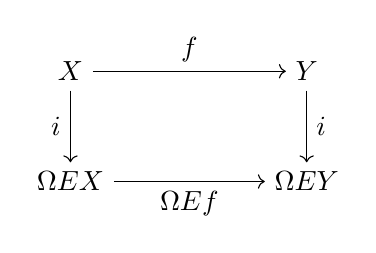
\begin{tikzpicture}[baseline=(current bounding box.center)]
\node (X) at (0,0) {$X$};
\node (Y) at (3,0) {$Y$};
\node (OX) at (0,-1.4) {$\Ox EX$};
\node (OY) at (3,-1.4) {$\Ox EY$};
\draw[->] (X)--node[above] {$f$} (Y);
\draw[->] (X)--node[left] {$i$} (OX);
\draw[->] (Y)--node[right] {$i$} (OY);
\draw[->] (OX)--node[below] {$\Ox Ef$} (OY);
\end{tikzpicture}
% \tag{1.9}
\end{equation}

$F:EX\to Y$ に対して,
\[
\Omega_0F=
\Ox F\circ i:\ X\xrightarrow{\ i\ }\Ox EX\xrightarrow{\ \Ox F\ }\Ox Y
\]
と書く. これは
\[
\Omega_0F(x)(t) = F(d_X(x,t))
\]
で直接に与えられる. \\
対応 $F\longmapsto \Omega_0F$ は,
$\map(EX,Y), \map(X,\Omega Y)$ のコンパクト部分集合
の間の同相を与え, \\
したがって, ホモトピー集合の間の次の全単射を誘導する.
\begin{equation}
% (1.10)
\Omega_0:\ [EX,Y]\xrightarrow{\ \cong\ }[X, \Ox Y].
\end{equation}
$[X,\Ox Y]$ に, \(\Omega Y\) loop 乗法による群演算を入れるとき, 
\(\Omega_0\) は群の同型である.\\
この演算は, $X$ が suspension $EX'$ のとき, 
上述の $+$ と一致する. このとき, 次の図式は可換である：
\begin{equation}
% (1.11)
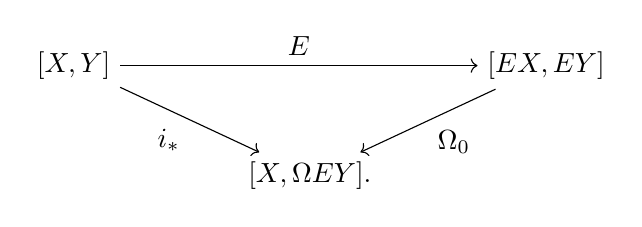
\begin{tikzpicture}[baseline=(current bounding box.center)]
\node (PX) at (-3,0) {$[X, Y]$};
\node (P1) at (3,0) {$[EX, EY]$};
\node (P2) at (0,-1.4) {$[X, \Ox EY].$};
\draw[->] (PX)--node[above] {$E$} (P1);
\draw[->] (PX)--node[below left] {$i_*$} (P2);
\draw[->] (P1)--node[below right] {$\Omega_0$} (P2);
\end{tikzpicture}
\end{equation}

$f:X\to Y,\ g:EY\to Z,\ h:Z\to W$ と,
そのホモトピー類 $\alpha=[f],\ \beta=[g],\ \gamma=[h]$ に対して, \\
以下が成り立つ：
\begin{equation}
% (1.12)
\begin{aligned}
\Omega_0(g\circ Ef)&=\Omega_0 g\circ f, &
\Omega_0(h\circ g)&=\Ox h\circ \Omega_0 g,\\
\Omega_0(\beta\circ E\alpha)&=\Omega_0 \beta\circ \alpha, &
\Omega_0(\gamma\circ \beta)&=\Ox\gamma\circ \Omega_0\beta .
\end{aligned}
\end{equation}

$0\in[X, Y]$ を,
自明な写像 $X\to y_0\in Y$ の類とする. \\
% \subsection*{Secondary composition の定義}
$n\ge 0$ を整数とし, 
$\alpha\in[\Ex^n Y, Z]$, $\beta\in[X, Y]$, $\gamma\in[W, X]$ が,
\begin{equation}
% (1.13)
\alpha\circ \Ex^n\beta=0,\qquad \beta\circ \gamma=0
\end{equation}
を満たすものとする. 代表写像を, それぞれ,
\[
a:(\Ex^n Y,y_0)\to (Z,z_0),\quad
b:(X,x_0)\to (Y,y_0),\quad
c:(W,w_0)\to (X,x_0)
\]
とする. 
このとき, (1.13) の仮定から, それぞれの null homotopy
\[
A_t:(\Ex^n X,x_0)\to (Z,z_0),\qquad
B_t:(W,w_0)\to (Y,y_0),\qquad (0\le t\le 1)
\]
で, 次を満たすものが存在する. 
\[
A_0=a\circ \Ex^n b,\quad A_1(\Ex^n X)=z_0,\qquad
B_0=b\circ c,\quad B_1(W)=y_0.
\]
写像 $H:\ (\Ex^{n+1}W,w_0)\to (Z,z_0)$ を, 次で定める. 
\begin{equation}\label{eq:H-def}
% (1.14)
H(d(w,t))=
\begin{cases}
a\bigl(\Ex^n B_{2t-1}(w)\bigr), & \tfrac12\le t\le 1,\\[2mm]
A_{1-2t}\bigl(\Ex^n c(w)\bigr), & 0\le t\le \tfrac12.
\end{cases}
\end{equation}
ここで,
$d:\Ex^n W\times I\to \Ex^{n+1}W$ は,
\(E^{n+1}W= E(E^n W)\) を定める等化写像で, 
$w\in \Ex^n W$ とする.\\
$H$ は well-defined で, 連続であり, 
$A_t,B_t$ の取り方と, $a,b,c$ に依存する. 

%\begin{definition}
\emph{secondary composition}
\[
\{\alpha,\ \Ex^n\beta,\ \Ex^n\gamma\}_n\ \subset\ [\Ex^{n+1}W, Z]
\]
を, 上の方法で得られる写像 $H$ の, 
ホモトピー類全体の集合として定める. 
%\end{definition}

ここで, 以下の記法を用いる. 
$A\subset[Y, Z]$, $B\subset[X, Y]$ に対し,
\[
A\circ B=\{\ \alpha\circ\beta\mid \alpha\in A,\ \beta\in B\ \}
\]
と書く. また, $A_1,A_2\subset[\Ex X, Y]$ に対し,
\[
A_1+A_2=\{\ \alpha_1+\alpha_2\mid \alpha_i\in A_i\ \}
\]
とする. 

\begin{lemma}\label{lem:double-coset}
% Lem1.1
$\{\alpha,\Ex^n\beta,\Ex^n\gamma\}_n$ は,
$[\Ex^{n+1}W, Z]$ の中で,
次の部分群の double coset である.
\[
[\Ex^{n+1}X, Z]\circ \Ex^{n+1}\gamma, \qquad
\alpha\circ \Ex^n\!\bigl([\Ex W, Y]\bigr).
\]
$[\Ex^{n+1}W, Z]$ が可換,
特に, $n>0$ あるいは, $W=\Ex W'$ または, $Z=\Omega Z'$ のとき, \\
\(
\{\alpha,\Ex^n\beta,\Ex^n\gamma\}_n
\)
は, 次の部分群の coset である.
\[
[\Ex^{n+1}X, Z]\circ \Ex^{n+1}\gamma \ +\ 
\alpha\circ \Ex^n\!\bigl([\Ex W, Y]\bigr).
\]
\end{lemma}

Proof.\
(1.14) の写像が,
\(a,b,c\) の取り方によらず, 互いに homotopic になることは, 
簡単に確かめられる.\\
$H$ を上で定義されたものとし, \\
\(H'\) を
\(a\circ E^n b,\ b\circ c\) の, 
別の null-homotopy $A'_t,\ B'_t$ を用いて定義されたものとする.
\newpage

\[
F:(\Ex^{n+1}X,x_0)\to (Z,z_0), \quad
G:(\Ex W,w_0)\to (Y,y_0)
\]
を, 次で定義する.
\[
F(d_{E^{n}Z}(x,t))\equiv\left\{
\begin{array}{ll}
A_{2t-1}(x), & \frac{1}{2} \leq t \leq 1, \\
A'_{1-2t}(x), & 0 \leq t \leq \frac{1}{2}, \\
\end{array}\right.
\]
\[
G(d_{W}(w,t))\equiv\left\{
\begin{array}{ll}
B'_{2t-1}(w), & \frac{1}{2} \leq t \leq 1, \\
B_{1-2t}(w), & 0 \leq t \leq \frac{1}{2}. \\
\end{array}\right.
\]
ここで,
\(x\in E^n X,\ w\in W\).
このとき,
\[
H'\ \simeq\ F\circ \Ex^{n+1}c\ +\ \bigl(H\ +\ a\circ \Ex^n G\circ \sigma\bigr)
\]
が確かめられる. 
ここで, 
$\sigma:\Ex^{n+1}W=W\ \wedge\ S^{n+1}\to \Ex^{n+1}W$ は,
\[
\sigma\bigl(\phi(w,\psi_{n+1}(t_1,\ldots,t_n,t))\bigr)=\phi(w, \psi_{n+1}(t, t_1,\ldots,t_n))
\]
で与えられる自己同相である. 対応
\[
\psi_{n+1}(t_1,\cdots,t_n, t) \longleftrightarrow
\psi_{n+1}(t,t_1,\cdots,t_n)
\]
は, $S^{n}$ 上の次数 $(-1)^n$ の同相写像なので,
\(\sigma\) は,
\(E^{n+1}W\) の恒等写像か,
反転写像に homotopic である.\\
よって,
\[
[H'] = [F]\circ E^{n+1}\gamma + 
([H] \pm \alpha \circ E^n [G])
\]
であり,
従って $H$ と $H'$ は, 
同じ double coset に属する. \\
逆に, \([H]\) と同じ double coset に属する \([E^{n+1}W,Z]\) の任意の元は,
ある写像
\[
F':(E^{n+1}X,x_0)\to(Z,z_0),\qquad
G':(EW, w_0)\to (Y,y_0)
\]
によって, 次の写像で表される.
\[
F'\circ E^{n+1}c + (H + a\circ E^n G'\circ \sigma).
\]
ここで,
\[
A'_t(x)=
\begin{cases}
F'(d_{E^n X}(x,2-2t)),& \tfrac12\le t\le 1,\\
A_{2t}(x),& 0\le t\le \tfrac12,
\end{cases}
\qquad
B'_t(w)=
\begin{cases}
G'(d_W(w,2t-1)),& \tfrac12\le t\le 1,\\
B_{2t}(w),& 0\le t\le \tfrac12,
\end{cases}
\]
と定めることで,
\(a\circ E^n b,\ b\circ c\) の null homotopy が得られる.\\
この \(A'_t,\ B'_t\) を用いて, $H'$ を作ると,
次が成り立つ.
\[
H'\ \simeq\ F'\circ \Ex^{n+1}c\ +\ (H+a\circ \Ex^n G').
\]
よって,
\([H]\)
の同じ double coset に属する任意の元は,
(1.14) の写像で表される.\\
以上から,
\(
\{\alpha,\ \Ex^n\beta,\ \Ex^n\gamma\}_n
\)
は,\\
\([E^{n+1}X,Z]\circ E^{n+1}\gamma,\ \alpha\circ E^n([EW,Y])\)
の double coset になることが示された. \\
Lemma の後半は容易に分かる.
\qed

\(n\ge m\ge 0\) とする.
(1.14) の写像は,
\(a,\ E^{n-m}b,\ E^{n-m}c\) と, \\
homotopy \(A_t,\ E^{n-m}B_t\)
を使って構成したものとみなせる.
これから, 次が成り立つ.
\begin{equation}\label{eq:split-m}
% (1.15)
\{\alpha,\ \Ex^n\beta,\ \Ex^n\gamma\}_n
\ \subset\
\bigl\{\alpha,\ \Ex^{m}(E^{n-m}\beta),\ E^{m}(E^{n-m}\gamma)\bigr\}_m .
\end{equation}

% \paragraph*{記法 ($n=0$ の場合) }
$n=0$ のときは, 
簡単に $\{\alpha,\beta,\gamma\}_0$ を,
$\{\alpha,\beta,\gamma\} \subset[\Ex W, X]$ と書く. 

\begin{proposition}[]\label{prop:1-2}
\leavevmode
\begin{enumerate}
\item[$0).$] $\alpha$, $\beta$, $\gamma$ のうち, いずれかが $0$ なら,
\[
\{\alpha,\ \Ex^n\beta,\ \Ex^n\gamma\}_n\equiv0.
\]
\item[$i).$] $\alpha\circ \Ex^n\beta=\beta\circ\gamma=0$ のとき,
\[
\{\alpha,\ \Ex^n\beta,\ \Ex^n\gamma\}_n\circ\Ex^{n+1}\delta\ \subset\ \{\alpha,\Ex^n \beta, \Ex^n(\gamma\circ\delta)\}_n.
\]
\item[$ii).$] $\alpha\circ \Ex^n\beta=\beta\circ\gamma\circ\delta=0$ のとき,
\[
\{\alpha,\ \Ex^n\beta,\ \Ex^n(\gamma\circ\delta)\}_n\ \subset\ \{\alpha,\ \Ex^n(\beta\circ\gamma),\ \Ex^n\delta\}_n .
\]
\item[$iii).$] $\alpha\circ\Ex^n\beta\circ\Ex^n\gamma=\gamma\circ\delta=0$ なら,
\[
\{\alpha\circ\Ex^n\beta,\ \Ex^n\gamma,\ \Ex^n\delta\}_n\ \subset\ \{\alpha,\ \Ex^n(\beta\circ\gamma),\ \Ex^n\delta\}_n .
\]
\item[$iv).$] $\beta\circ\Ex^n\gamma=\gamma\circ\delta=0$ のとき,
\[
\alpha\circ\{\beta,\ \Ex^n\gamma,\ \Ex^n\delta\}_n\ \subset\ \{\alpha\circ\beta,\ \Ex^n\gamma,\ \Ex^n\delta\}_n .
\]
\end{enumerate}
\end{proposition}

Proof.\ 
0). $\alpha$ または $\beta$ が $0$ のときは, 
それぞれ, $A_t$ または $B_t$ を,
null-homotopy に取ることができる. \\
このとき, (1.14) の写像 \(H\) の類は 
\(\alpha\circ E^n([EW,Y])\) に属する.
よって, \(\todai[n]{\alpha, E^n\beta, E^n\gamma}\equiv0\).\\
\(\gamma=0\) の場合も同様に示される.

i). 
\(a,b,c,A_t,B_t\) から, (1.14) により定義された写像 \(H\)
を考える.\\
この写像の類は 
\(\todai[n]{\alpha, E^n\beta, E^n\gamma}\)
に属する.\\
\(\delta\) を表す写像を \(d\) とする.\\
\(a,b,c\circ d, A_t, B_t\circ d\) から, (1.14) により定義された写像を \(H'\)
とすると,\\
この類は, \(\todai[n]{\alpha, E^n\beta, E^n(\gamma\circ\delta)}\)
に属し, 
\(H'=H\circ E^{n+1}d\) が成り立つ.\\
以上で i) が示された.

ii), iii), iv) も同様に示される.
\qed


\begin{proposition}\label{prop:1-3}
任意の $n\ge 0$ に対し,
\[
-\Omega_0\bigl\{\alpha,\ \Ex^{n+1}\beta,\ \Ex^{n+1}\gamma\bigr\}_{n+1}
=
\bigl\{\Omega_0\alpha,\ \Ex^{n}\beta,\ \Ex^{n}\gamma\bigr\}_n \ ,
\]
\[
-\Ex\{\alpha,\ \Ex^n\beta,\ \Ex^n\gamma\}_n
\subset
\bigl\{E\alpha,\ \Ex^{n+1}\beta,\ \Ex^{n+1}\gamma\bigr\}_{n+1}.
\]
\end{proposition}

Proof.\
$a,b,c$ をそれぞれ $\alpha,\beta,\gamma$ の代表とする.\\
\(\todai[n+1]{\alpha, E^{n+1}\beta, E^{n+1}\gamma}\) 
の任意の元は, 次の写像 \(H:E^{n+2}W\to Z\)
で表される.
\[
H(d_{ER}(d_R(w,s),t))=
\begin{cases}
a(\Ex^{n+1}B_{2t-1}(d_R(w,s))), 
& \tfrac12\le t\le 1,\\[2mm]
A_{1-2t}(\Ex^{n+1}c(d_R(w,s))), 
& 0\le t\le \tfrac12,
\end{cases}
\]
ここで,
\(w\in R = E^n W\)
で,
\(A_t,\ B_t\) 
は, それぞれ,
\(a\circ E^{n+1}b,\ b\circ c\)
の null-homotopy とする.\\
\(E^2 R\) を定義する等化写像
\(\phi:R\times S^2\to R\wedge S^2 = E^2 R\)
に対して,
\[
d_{ER}(d_R(w,s),t) = \phi(w, \psi_2(s, t)).
\]
\(\sigma:E^{n+2}W\to E^{n+2}W\)
を, 次で与えられる同相写像とする.
\[
\sigma(d_{ER}(d_R(w,s),t))
= d_{ER}(d_R(w,t), s).
\]
このとき, Lem1.1の証明で見たように,
\([H\circ \sigma] = -[H]\) である.\\
(1.12) と \(\Omega_0\) の定義により,
\[
\Omega_0(H\circ \sigma)(d_R(w,t))=
\begin{cases}
\Omega_0 a(\Ex^{n}B_{2t-1}(w)), 
& \tfrac12\le t\le 1,\\[2mm]
\Omega_0 A_{1-2t}(\Ex^{n}c(w)), 
& 0\le t\le \tfrac12.
\end{cases}
\]
よって,
\(\Omega_0[H\circ \sigma]\)
は, 
\(\todai[n]{\Omega_0\alpha, E^n\beta, E^n\gamma}\)
に属する.\\
逆に, 
\(\todai[n]{\Omega_0\alpha, E^n\beta, E^n\gamma}\)
の任意の元は,
\(\Omega_0\) が同相なので,
上のような \(\Omega_0(H\circ \sigma)\) で表される.\\
以上で, この Prop の最初の等式が証明された.

\(\iota\) を, canonical injection \(i:Z\to \Omega EZ\)
の類とする.
(1.11), Prop1.2 iv) により,
\[
\begin{align*}
  -E\todai[n]{\alpha, E^n\beta, E^n\gamma}
  & = -\Omega_0^{-1}(\iota \circ \todai[n]{\alpha, E^n\beta, E^n\gamma})
  \subset -\Omega_0^{-1}\todai[n]{\iota\circ\alpha, E^n\beta, E^n\gamma}\\
  & = \todai[n+1]{\Omega_0^{-1}\circ\iota\circ\alpha, E^{n+1}\beta, E^{n+1}\gamma}
  = \todai[n+1]{E\alpha, E^{n+1}\beta, E^{n+1}\gamma}.
\end{align*}
\]
これで, Prop1.3 の証明が完了した.
\qed

\begin{proposition}\label{prop:1-4}
$\alpha\circ \Ex^n\beta=\beta\circ\gamma=\gamma\circ\delta=0$ のとき, 
次が成り立つ.
\[
\{\alpha,\ \Ex^n\beta,\ \Ex^n\gamma\}_n\circ\Ex^{n+1}\delta
=
(-1)^{n+1}\bigl(\alpha\circ \Ex^n\{\beta,\ \gamma,\ \delta\}\bigr).
\]
\end{proposition}

Proof.\
\([a]=\alpha,\ [b]=\beta,\ [c]=\gamma,\ [d]=\delta\)
とし,\\
\(A_{t},\ B_{t},\ C_{t}\)
をそれぞれ,
\( a\circ\Ex^{n}b,\ b\circ c,\ c\circ d\)
のnull homotopyとする.\\
このとき, 
\(H:E^{n+1}V\to Z\) を 
\[
H(d_{E^n V}(s, t)) = \left\{
\begin{array}{ll}
  A_{1-2t}(E^n c(E^n d(s))),
  & 0\leq t \leq \frac{1}{2},\\
  a(E^n B_{2t-1}(E^n d(s))), 
  & \frac{1}{2} \leq t \leq 1.  
\end{array}
\right.
\]
で, 定義すると,
\([H]\) は 
\(\todai[n]{\alpha, E^n\beta, E^n\gamma}\circ E^{n+1}\delta\)
の元を表す.\\
homotopy
\(H_{u}:(\Ex^{n+1}V,v_0) \longrightarrow (Z,z_0)\)
を, 次で定義する.
\[
H_{u}(d_{\Ex^{n}V}(s,t))\equiv\left\{
\begin{array}{ll}
A_{1-2t}(\Ex^{n}C_{2u(1-2t)}(s)), &
0\leq t \leq \frac{1}{2},\ 0\leq u \leq \frac{1}{2}, \\
A_{(2-2u)(1-2t)}(\Ex^{n}C_{1-2t}(s)), &
0\leq t \leq \frac{1}{2},\ \frac{1}{2} \leq u \leq 1, \\
a(\Ex^{n}B_{2t-1}(\Ex^{n}d(s))), &
\frac{1}{2} \leq t \leq 1.
\end{array}\right.
\]
\(\sigma:\Ex^{n+1}V\to\Ex^{n+1}V \notag\)
を, 次で定義される同相写像とする.
\[
\sigma(\phi_{V,S^{n+1}}(v,\psi_{n+1}(t_{1},\cdots,t_{n},t))) :=
\phi_{V,S^{n+1}}(v,\psi_{n+1}(1-t,t_{1},\cdots,t_{n})).
\]
また, 写像 \(K:EV\to Y\) を次で定義する.
\[
K(d_{V}(v, t)) = \left\{
\begin{array}{ll}
  B_{1-2t}(d(v)),
  & 0\leq t \leq \frac{1}{2},\\
  b(C_{2t-1}(v)), 
  & \frac{1}{2} \leq t \leq 1.  
\end{array}
\right.
\]
このとき,
\(K\) は \(\toda{\beta, \gamma, \delta}\) の元を表し,
\(H_u\)
は, \(H\) と \(a\circ E^n K \circ \sigma\) 
の間の homotopy である.\\
\(\sigma\) の degree が \((-1)^{n+1}\) なので,
\([H] = [a\circ E^n K\circ \sigma]\)
は,
\((-1)^{n+1}(\alpha\circ E^n\toda{\beta, \gamma, \delta})\)
の元を表す.\\
逆に, 
\((-1)^{n+1}(\alpha\circ E^n\toda{\beta, \gamma, \delta})\)
の任意の元は,\\
適当な homotopy \(B_t,\ C_t\) によって,
上のような合成 \(a\circ E^n K\circ \sigma\)
で表される.\\
homotopy \(H_{1-u}\) を使うことにより,
\[
[a\circ E^n K\circ\sigma]
\in \todai[n]{\alpha, E^n\beta, E^n\gamma}\circ E^{n+1}\delta
\]
が示される.
以上で, Prop1.4 の証明が完了した.
\qed

% --- (続き) p.12–13 ---

\begin{proposition}[]\label{prop:1-5}
$\alpha,\beta,\gamma,\delta,\varepsilon$ を,
\[
\alpha\circ \beta=\beta\circ\gamma=\gamma\circ\delta=\delta\circ\varepsilon=0
\]
\[
0\in \alpha\circ\{\beta,\ \gamma,\ \delta\}, \ \ 0\in\{\beta,\ \gamma,\ \delta\}\circ\Ex\varepsilon
\]
を満たす元とする. このとき,
\[
\lambda\in\{\alpha,\beta,\gamma\},\quad
\mu\in\{\beta,\gamma,\delta\},\quad
\nu\in\{\gamma,\delta,\varepsilon\}
\]
を適当に選ぶことができ, それらは,
\[
\lambda\circ \Ex\delta=\alpha\circ \mu=0,\qquad
\beta\circ \nu=\mu\circ \Ex\varepsilon=0
\]
を満たし, 次の和は $0$ を含む. 
\[
\{\lambda,\ \Ex\delta,\ \Ex\varepsilon\}
\ +\
\{\alpha,\ \mu,\ \Ex\varepsilon\}
\ +\
\{\alpha,\ \beta,\ \nu\}.
\]
\end{proposition}

\noindent (要するに) 
\[
\{\{\alpha,\beta,\gamma\},\ E\delta,\ E\varepsilon\}
+\{\alpha,\ \{\beta,\gamma,\delta\},\ E\varepsilon\}
+\{\alpha,\ \beta,\ \{\gamma,\delta,\varepsilon\}\}
\equiv0 .
\]
このPropは [25]Th4.3(ii) の一般化で, 球面を位相空間に置き換えて, 
同様の証明をすることで得られる. 

\begin{proposition}[]\label{prop:1-6}
% Prop1.6
$\alpha,\alpha'\in[\Ex^n Y, Z]$, $\beta,\beta'\in[X, Y]$, 
$\gamma,\gamma'\in[W, X]$ とする. \\
$n\ge 1$ \emph{または} $W=\Ex W'$ の場合には,
\[
\{\alpha,\Ex^n\beta,\Ex^n\gamma\}_n
+
\{\alpha,\Ex^n\beta,\Ex^n\gamma'\}_n
\ \supset\
\{\alpha,\Ex^n\beta,\Ex^n(\gamma+\gamma')\}_n
\]
が成り立つ. 
$n\ge 1$ \emph{または} $\gamma=\Ex\gamma' \ (X=\Ex X',\ W=\Ex W')$ の場合には,
\[
\{\alpha,\Ex^n\beta,\Ex^n\gamma\}_n
+
\{\alpha,\Ex^n\beta',\Ex^n\gamma\}_n
\ =\
\{\alpha,\Ex^n(\beta+\beta'),\Ex^n\gamma\}_n,
\]
が成り立つ. $n\ge 1$ \emph{または} $\beta=\Ex\beta',\ \gamma=\Ex\gamma' \ (Y=\Ex Y',\ X=\Ex X',\ W=\Ex W')$ の場合には
\[
\{\alpha,\Ex^n\beta,\Ex^n\gamma\}_n
+
\{\alpha',\Ex^n\beta,\Ex^n\gamma\}_n
\ \supset\
\{\alpha+\alpha',\Ex^n\beta,\Ex^n\gamma\}_n
\]
が成り立つ. 
\end{proposition}

Proof.\
まず, 
\(n\ge1\) または \(W=EW'\) なので, 
\([\Ex^{n+1}W,Z]\) はアーベル群であることに注意する.

最後の関係式を示す. 
\(
\{\alpha+\alpha',\Ex^n\beta,\Ex^n\gamma\}_n
\)
は, 次の部分群の coset である. 
\[
(\alpha+\alpha')\circ \Ex^{n+1}\!\bigl([W, Y]\bigr) 
+ [\Ex^{n+1}X, Z]\circ \Ex^{n+1}\gamma.
\]
他方, 
\(
\{\alpha,\Ex^n\beta,\Ex^n\gamma\}_n + \{\alpha',\Ex^n\beta,\Ex^n\gamma\}_n
\)
は, 次の部分群の coset である.
\[
\alpha\circ E^{n+1}[W,X]
+ \alpha'\circ E^{n+1}[W,X]
+ [E^{n+1}X,Z].
\]
この群は, 次の元を含んでいる.
\[
(\alpha + \alpha') \circ E^{n+1}[W,X]
+ [E^[n+1]X,Z] \circ E^{n+1}\gamma.
\]
よって,
\(
\{\alpha+\alpha',\Ex^n\beta,\Ex^n\gamma\}_n
\)
と
\(
\{\alpha,\Ex^n\beta,\Ex^n\gamma\}_n + \{\alpha',\Ex^n\beta,\Ex^n\gamma\}_n
\)
が, 共通元を持つことを示せば十分.

定義に従って (1.14) から,
\(\todai[n]{\alpha, E^n\beta, E^n\gamma}\) と,
\(\todai[n]{\alpha', E^n\beta, E^n\gamma}\) を表す写像\\ 
$H,H':E^{n+1}W\to Z$ を構成する.\\
それぞれ, $a,b,c$ と, $a',b,c$
および, \(a\circ E^n b,\ a'\circ E^n b, b\circ c\)
の null-homotopy $A_t,\ A'_t,\ B_t$ を用いる. \\
\(\phi: E^{n-1}W\times S^2\to E^{n+1}W = E^{n-1}W\wedge S^2\)
を, \(E^{n+1}W = E^2 E^{n-1}W\) を定義する写像とする.\\
ここで, \(n=0\) のときは, \(E^{n-1}W = W'\) である.\\
\(\sigma:E^{n+1}W\to E^{n+1}W\) を,
\(\sigma(\phi(w, \psi_2(s, t)))
= \phi(w, \psi_2(t, s))\)
で定義される同相写像とする.\\
このとき,
\(\sigma\) は,
\(E^{n+1}W\) の反転写像と homotopic であり,\\
任意の \(H_0:(E^{n+1}W,w_0)\to(Z,z_0)\) に対して,
\([H_0\circ\sigma] = -[H_0]\) である.\\
$H'':(E^{n+1}W,w_0)\to(Z,z_0)$ を, 次で定義する.
\[
H''(\phi(w,\psi_2(s, t))) :=
\begin{cases}
H(\phi(w, \psi_2(2s, t))), & 0\le s\le \tfrac12,\\
H'(\phi(w, \psi_2(2s-1, t))), & \tfrac12\le s\le 1.
\end{cases}
\]
このとき, 
\(H''\circ \sigma = 
H\circ \sigma + H'\circ \sigma\)
であることと,\\
\(H''\) が
\(a+a',\ b,\ c\) と, homotopy \(A_t + A'_t,\ B_t\) 
から, (1.14) により構成されることが, 直接的に確かめられる.\\
したがって,
\[
[H] + [H'] = [H''] \in 
\todai[n]{\alpha + \alpha', E^n\beta, E^n\gamma}
\]
であり, 
\([H'']\) は求める共通元である.
以上より,
Prop1.6 の最後の関係式が証明された.\\
最初と2番目の関係式の証明は省略する.
\qed

% \subsection*{Mapping cone と extension/coextension}

基空間 $X$ 上の \emph{cone} \(CX\) を, 次で定義する.
\[
CX=(X\times I)/\bigl(X\times\{1\}\ \cup\ x_0\times I\bigr).
\]
$d'_X:X\times I\to CX$ を, \(CX\) を定義する等化写像とする.\\
対応 $x\longleftrightarrow d'_X(x,0)$ により, 
$X$ と $d'_X(X\times {0})$ を同一視する. 

$\beta\in[X, Y]$ と, その代表 $f:(X,x_0)\to(Y,y_0)$ を考える.\\
\(CX\) と \(Y\) の disjoint union \(Y \sqcup CX\)
において, \\
\(X\) と \(f\) による像を同一視した空間を,
\(Y\cup_f CX\) または, \(Y\cup_\beta CX\) で表す.\\
$Y\cup_f CX$ のホモトピー型は, \(\beta\) の代表 $f$ の選び方によらない. 

\(\overline{\alpha}\in[Y\cup_\beta CX, Z]\)
は, \(\overline{\alpha}\) を表す写像 \(g\)
に対して, 
制限 \(g|_{Y}\) が \(\alpha\in[Y,Z]\) を表すとき,\\
$\alpha$ の \emph{extension} と呼ぶ.

\(\widetilde{\gamma}\in[EW,Y\cup_\beta CX]\)
に対して, \(\widetilde{\gamma}\) を表す写像 
\(h:EW\to Y\cup_\beta CX\)
が, 次の条件を満たすとする.
\[
h(d_W(w, t)) \left\{
\begin{array}{ll}
= d'_X(c(w), 1-2t), & 0 \leq t \leq \frac{1}{2}, \\
\in Y, & \frac{1}{2} \leq t \leq 1. \\
\end{array}\right.
\]
ここで, \(c:W\to X\) は \(\gamma\in[W,X]\) を表す写像とする.
このとき, \(\widetilde{\gamma}\) を \(\gamma\) の \emph{coextension} と呼ぶ.\\
extension $\overline\alpha$ が存在するための必要十分条件は,
$\alpha\circ \beta=0$ であり,\\
coextension $\widetilde{\gamma}$ が存在するための必要十分条件は,
$\beta\circ\gamma=0$ である. 

次の同一視を使用する.
\begin{equation}\label{eq:cone-susp}
% (1.16)
\Ex^n(Y\cup_\beta CX)\ =\ 
\Ex^nY\ \cup_{\beta'}\ C\Ex^n X,\quad \beta'=\Ex^n \beta.
\end{equation}
ここで, 対応は
\[
\phi(d'_X(x,t),\psi_n(t_1,\ldots,t_n))\longleftrightarrow d'_Z(\phi'(x,\psi_n(t_1,\ldots,t_n)),t)
\]
により与えられ, $Z=\Ex^n X$ であり, \\
$\phi, \ \phi'$ は, それぞれ, 
$\Ex^n(Y\cup_\beta CX)=(Y\cup_\beta CX)\wedge S^n$ と,
$\Ex^n X=X\wedge S^n$ を定義する写像である. 

\begin{proposition}[]\label{prop:1-7}
\(\alpha\in[E^nY, Z],\ \beta\in[X,Y],\ \gamma\in[W,X]\) に対して,
  $\alpha\circ \Ex^n\beta=\beta\circ\gamma=0$ を仮定する. \\
$\alpha$ の extension $\overline\alpha\in[\Ex^n(Y\cup_\beta CX), Z]$ と,
$\gamma$ の coextension $\widetilde\gamma\in[EW, Y\cup_\beta CX]$ を考える. 
このとき,
\[
\{\ \overline\alpha\circ \Ex^n\widetilde\gamma\ \}
= (-1)^n\{\alpha,\ \Ex^n\beta,\ \Ex^n\gamma\}_n.
\]
\end{proposition}

Proof.\
\(\beta\) を表す写像 \(b = f\) に対して, 
\(B_t\) を \(b\circ c\) の null-homotopy とする.\\
$h:EW\to Y\cup_f CX$ を,
次で定める.
\[
h\bigl(d_W(w,t)\bigr)=
\begin{cases}
d'_X(c(w),1-2t), & 0\le t\le \tfrac12,\\
B_{2t-1}(w), & \tfrac12\le t\le 1.
\end{cases}
\]
また, \(A_0 = a\circ E^n b = (g|_{E^n Y})\circ E^n f\)
を満たす null-homotopy \(A_t\) に対して,\\
\(\overline{\alpha}\) の代表 \(g\) が,
\(g(d'_X(x, t)) = A_t(x)\) を満たす.\\
Lem1.1 の証明における \(E^{n+1}W\) の同相写像 \(\sigma\) に対して,\\
(1.14) により与えられた写像 \(H\) に対して,
\(g\circ E^n h = H\circ \sigma^{-1}\) が成り立つことが,
直接的に確かめられる.\\
よって,
\(g\circ E^n h\) の類 \(\overline{\alpha}\circ E^n\widetilde{\gamma}\)
は, \((-1)^n\todai[n]{\alpha, E^n\beta, E^n\gamma}\) に属する.\\
逆に,
\((-1)^n\todai[n]{\alpha, E^n\beta, E^n\gamma}\)
の任意の元は, 
\(g\circ E^n h = H\circ\sigma^{-1}\)
の形の写像で表される.\\
以上で, Prop1.7 が証明された.
\qed

% --- (続き) p.14–15 ---

\begin{proposition}\label{prop:1-8}
$\alpha,\beta,\gamma$ は, Prop$1.7$ と同様とする. \\
$\widetilde{\beta}\in[\Ex^{n+1}X, Z\cup_\alpha C\Ex^nY]$ を,
$E^n\beta$ の \emph{coextension} とするとき,
次が成り立つ.
\[
\bigl\{\ \widetilde{\beta}\circ\Ex^{n+1}\gamma\ \bigr\}
\ =\
-\,i_*\bigl\{\alpha,\ \Ex^n\beta,\ \Ex^n\gamma\bigr\}_n.
\]
ここで, $i:Z\hookrightarrow Z\cup_\alpha C\Ex^nY$ は,
自然な包含写像である. 
\end{proposition}

Proof.\
次の式で与えられる homotopy  
\(H_s:(E^{n+1}W,w_0)\to (Z\cup_\alpha CE^n Y, z_0)\)
を考える.
\[
H_s\bigl(d(w,t)\bigr)=
\begin{cases}
d'_V\!\left(E^nB_{s(1-2t)}(w),\ (1-s)(1-2t)\right), & 0\le t\le \tfrac12,\\
A_{2t-1}\!\left(E^n c(w)\right), & \tfrac12\le t\le 1.
\end{cases}
\]
ここで, (1.14) と同じ記号を用い, \(V= E^n Y\) とする.\\
(1.14) により与えられる写像 \(H\) に対して, 
\(H_1 = -H\) であることと,\\
\(H_0\) が 
\(\widetilde{\beta}\circ E^{n+1}\gamma\)
を表すことが, 
直接的に確かめられる.\\
以上で, Prop1.8 が証明された.
\qed

\medskip

Lem1.1 と \(i_*(\alpha) = 0\) により,\\
\(-i_*\todai[n]{\alpha, E^n\beta, E^n\gamma}\) は, 
\(i_*[E^{n+1}X, Z]\circ E^{n+1}\gamma\)
の coset であることに注意する.

\begin{equation}\label{eq:p-def}
% (1.17)
p:X\cup_\gamma CW\to EW
\end{equation}
を, 次で与えらえる写像とする.
\[
p(d'_W(w, t)) = d_W(w, t),\qquad
p(X) = x_0.
\]
このとき,
\(p\) は \(X\) を一点につぶす写像であり, 次が成り立つ.
\begin{equation}\label{eq:p-star}
% (1.18)
p_*(\widetilde{\delta})=E\delta,
\quad\text{for a coextension }\ 
\widetilde{\delta}\in[EV, X\cup_\gamma CW]
\text{ of }\delta\in[V, W].
\end{equation}

\begin{proposition}\label{prop:1-9}
% Prop1.9
$\alpha,\beta,\gamma$ は, Prop$1.7$ と同様とする. \\
$\overline\beta\in[X\cup_\gamma CW, Y]$ を $\beta$ の \emph{extension} とする. 
このとき,
ある $\lambda\in[\Ex^{n+1}W, Z]$ が存在して, 次を満たす.
\[
(\Ex^n p)^*\lambda=\alpha\circ \Ex^n\overline\beta.
\]
このような $\lambda$ 全体の集合は,
\(
[\Ex^{n+1}X, Z]\circ \Ex^{n+1}\gamma
\)
の coset であり, 特に次が成り立つ.
\[
\{\lambda\}\ \subset\ \{\alpha,\ \Ex^n\beta,\ \Ex^n\gamma\}_n .
\]
逆に, $\{\alpha,\Ex^n\beta,\Ex^n\gamma\}_n$ の任意の元 $\lambda$ に対し, 
適当な extension $\overline\beta$ が存在して,
次が成り立つ.
\[
(\Ex^n p)^*\lambda=\alpha\circ \Ex^n\overline\beta.
\]
\end{proposition}

Proof.\
\(\alpha\circ E^n\overline{\beta}\) を表す写像 
\(G:E^n(X\cup_\gamma CW)\to Z\) は,
次の形で与えられる.
\[
\begin{cases}
  G(x) = a(E^n b(x)), & x \in E^n X,\\
  G(d'_V(w, t)) = a(E^n B_t(w)), & w \in E^n W = V,\ t \in I.
\end{cases}
\]
ここで,
\(a,\ b,\ c\) はそれぞれ, \(\alpha,\ \beta,\ \gamma\) を表し,
\(B_t\) は \(b\circ c\) の null-homotopy である.\\
\(\alpha\circ E^n\beta = 0\) なので,
制限 \(G|_{E^n X}\) は null-homotopic であり,\\
homotopy extension theorem により, 
homotopy \(G_s:E^n(X\cup_\gamma CW) \to Z\)
が存在し, 次を満たす.
\[
G_0 = G,\qquad 
G_1(E^n X) = z_0.
\]
このとき,
\(H_1\circ E^n p = G_1\) を満たす写像 
\(H_1 : E^{n+1}W \to Z\)
が一意的に存在する.\\
よって,
\(H_1\) の類 \(\lambda\) は, 
条件 \((E^n p)^*\lambda = \alpha\circ E^n\beta\)
を満たす.\\
さらに, 
\((E^n p)^*\lambda = \alpha\circ E^n\beta\)
を満たす任意の元は, 
この方法で与えられる写像 \(H_1\) により表される.\\
\(A_t = G_t|_{E^n X}\) とするとき,
\(A_t\) は \(a\circ E^n b\) の null-homotopy である.\\
次で与えられる homotopy 
$H_s:E^{n+1}W\to Z$ を考える.
\[
H_s\bigl(d_V(w,t)\bigr)=
\begin{cases}
A_{1-2t}\!\left(E^n c(w)\right), 
& 0\le t\le \dfrac{1-s}{2},\\
G_s\!\left(d'_V\!\left(w,\dfrac{2t-1+s}{1+s}\right)\right), 
& \dfrac{1-s}{2}\le t\le 1.
\end{cases}
\]
このとき, 
$H_s$ は $H_1$ と $H_0= (1.14) \text{ の }H$ の間の homotopy になる. \\
よって,
\(\lambda = [H_1] = [H]\) は,
\(\todai[n]{\alpha,\Ex^n\beta,\Ex^n\gamma}\) に属する.\\
上の議論の中で,
homotopy \(B_t\)
を固定して,
\(a\circ E^n b\) の null-homotopy \(A_t\) は任意に取り換える.\\
このとき,
Lem1.1 の証明の中でみたのと同様にして,
集合 \(\gen{\lambda}\) は,
\([E^{n+1}X, Z]\circ E^{n+1}\gamma\) の coset である.\\
さらに,
\(B_t\) を取り換えることにより,
\(\gen{\lambda}\) は
\(\todai[n]{\alpha, E^n\beta, E^n\gamma}\)
全体を走る.\\
以上で, Prop1.9 が証明された. 
\quad






\end{document}
